\chapter{Quantum Estimation}
% Section on density operator
In this chapter we identify the anatomy of the metrology problem and formulate it
in the language of quantum channels and statistical inference. Once this is done we obtain a generic recipe to obtain POVM independent
precision bounds.
\section{Statistical Inference}
\subsection{Estimators}
Any experiment one realizes has an underlying probability distribution over some set $\chi$ that representes the
possible outcomes, specified by the laboratory conditions e.g. temperature, pressure, instrumental precision, initial state and
represented by an element in some parameter space $\Theta$; our objective
is to study this unknown distribution from the experimental results, identifying it \textbf{as precisely as possible} i.e. we have a problem of
statistical inference. Below we present the basic structure of the \textbf{local estimation framework} following \cite{cover_elements_2006,paris_quantum_2009}, its essence is the assumption that the
distribution of study is a member of a known parametric family of probability distributions $\{p(x;\theta)\}_{\theta \in \Theta}$ from which we
must identify the particular $\theta$ that corresponds to our experiment via samples. From this is clear that we need a rule
to go from the sample to the parameter space and that its properties will allow us to study precision, this is the notion that the following
definition seeks to capture.

\begin{definition}
  Given a family $\{p_{\theta}(x)\}_{\theta \in \Theta}$ of probability distributions over some set $\chi$, we call an estimator for $\theta$ a
  sample of size $n$ a function $T:\chi^{n} \to \Theta$. Assuming $\Theta \subseteq \mathds{R}$:
  \begin{itemize}
  \item The difference $T - \theta$ is called \textbf{the error} of the estimator, note this is a random variable
  \item The expected value of the error is called \textbf{the bias}, and if it is zero we say the estimator is \textbf{unbiased}.
  \item Let  $X_{1}, ..., X_{n} \sim p_{\theta}$ be i.i.d random variables, $E[(T(X_{1}, ..., X_{n})-\theta)^{2}]$ is called the \textbf{Mean Square Error} (MSE) of the estimator.
  \item An estimator $T_{1}$ is said to \textbf{dominate} another one $T_{2}$ if its MSE is less than or equal for all $\theta \in \Theta$.

  \end{itemize}
\end{definition}

The MSE is the figure of merit that classifies the estimator $T$, and if it is unbiased we can identify it with $\var{T}$ so that
our credence on $T(x_{1}, ... x_{n})$ is codified in it. We give this last statement a concrete operational meaning through
Chebyshev's inequality:

\begin{theorem}
  Let X be a random variable with finite non-zero variance $\sigma^{2}$ and expected value $\mu$. For any real $k$ the probability of the
  difference between $X$ and $\mu$ being greater than $k\sigma$ is \cite{feller1971introduction}:
$$
P(|X-\mu|\geq k\sigma)\leq \frac{1}{k^{2}}
$$
\end{theorem}

The smaller the variance of $T$ the less likely it is for the difference between $T$ and the actual value $\theta$ to be greater than
$\var{T}$.

\subsection{The Fisher Information}
When one characterizes a measurement apparatus for a quantity $X$ a key property is how \textbf{sensible} it is i.e. given two values  of $X$,
$x$ and $x'$, what is the smallest $\Delta X = |x-x'|$ such that it can differentiate between the two. For estimators there is a similar
connection between a notion of sensitivity and its variance, given by the \textbf{Fisher Information} and the \textbf{Cram\'er-Rao bound}
respectevely.

\begin{definition}
  For a parametric family of probability distributions $\{p_{\theta}\}_{\theta \in \Theta}$ we define the \textbf{Fisher Information} (FI)
  as
  \begin{equation}
    F(\theta) = E\left[\left(\frac{\partial}{\partial \theta}\log{p_{\theta}(x)} \right)^{2}\right] = \int dx \hspace{0.1cm} \frac{(\partial_{\theta} p_{\theta}(x))^{2}}{p_{\theta}(x)}
  \end{equation}
\end{definition}


\begin{theorem}
  The MSE of an unbiased estimator $T$ of the parameter $\theta$ is bounded by
  \begin{equation}
    \var{T}\geq \frac{1}{F(\theta)}.
  \end{equation}
  This inequality is called the \textbf{Cram\'e-Rao bound} (CRB).
\end{theorem}

We say an estimator is \textbf{CR-efficient} if it saturates the CRB \cite{cover_elements_2006,wiseman_quantum_2010}. Note that the CR bound
depends on the family of probability distributions and its parametrization at a given point, not on the estimator. The FI \textbf{quantifies the
  amount of information about the parameter contained in the actual probability distribution} by describing the limits on the amount of
creedence we could assign to \textbf{any} estimation of the parameter $\theta$. The question now is whether the CRB is tight i.e. if there
always exists a CR-efficient estimator, the next theorem shows this is the case asymptotycally.

\begin{definition}
  Given a probability distribution $p_{\theta}$ where $\theta$ is a parameter, we define the \textbf{likelihood} of a sample $\{x_{1},...,x_{n}\}$
  as

  \begin{equation*}
    f_{\theta}(x_{1},...,x_{n}) = \prod_{k=1}^{n}p_{\theta}(x_{k}).
  \end{equation*}

  and the \textbf{Maximum Likelihood Estimator} (MLE)  $\hat{\theta}_{ML} : \chi^{n} \to \mathds{R}$ as
  \begin{equation*}
    \hat{\theta}_{ML}(x_{1}, ..., x_{n}) = \underset{\theta}{\text{arg\hspace{0.05cm}max}}\hspace{0.1cm} f_{\theta}(x_{1},...,x_{n})
  \end{equation*}

\end{definition}

essentially the likelihood measures how probable is to find a given sample provided a value of theta, and the MLE proposes as estimation the
value of the parameter for which this sample is most likely.

\begin{theorem}
The MLE saturates the CRB asymptotically \cite{kay1993fundamentals}.
\end{theorem}

\section{Characterization of Quantum Channels}
Let $\varepsilon_{\gamma}$ be a quantum channel with an unknown $\gamma$ we seek to estimate through some measurement, for this we
need to define an input (initial) state $\rho_{0}$ and perform some measurements on the output. The particular way we measure will
correspond to choosing a POVM $\{\Pi_{x}\}$ that describes the statistics of the experiment. More concretly, the outcomes follow the distribution

\begin{equation}
  \wp(x|\gamma) = \Tr{\Pi_{x}\varepsilon_{\gamma}(\rho_{0})}
\end{equation}

and from it we must infer the value of $\gamma$; from this it is clear that what we got at hand
really is a problem about statistical inference, in which the family of distributions is induced by the POVM.
This reasoning shows all the parts of a \textbf{Metrology Protocol}:

\begin{enumerate}
  \item an initial state
  \item a channel with an unknown parameter one wants to estimate, producing output states $\rho_{\gamma} = \varepsilon_{\gamma}(\rho_{0})$

  \item a measurement strategy, whose statistics are described by a POVM
  \item an estimator producing an estimate $\tilde\gamma$.
\end{enumerate}
in figure \ref{fig:metrology_scheme} this is represented.

\begin{figure}[h]
  \centering
  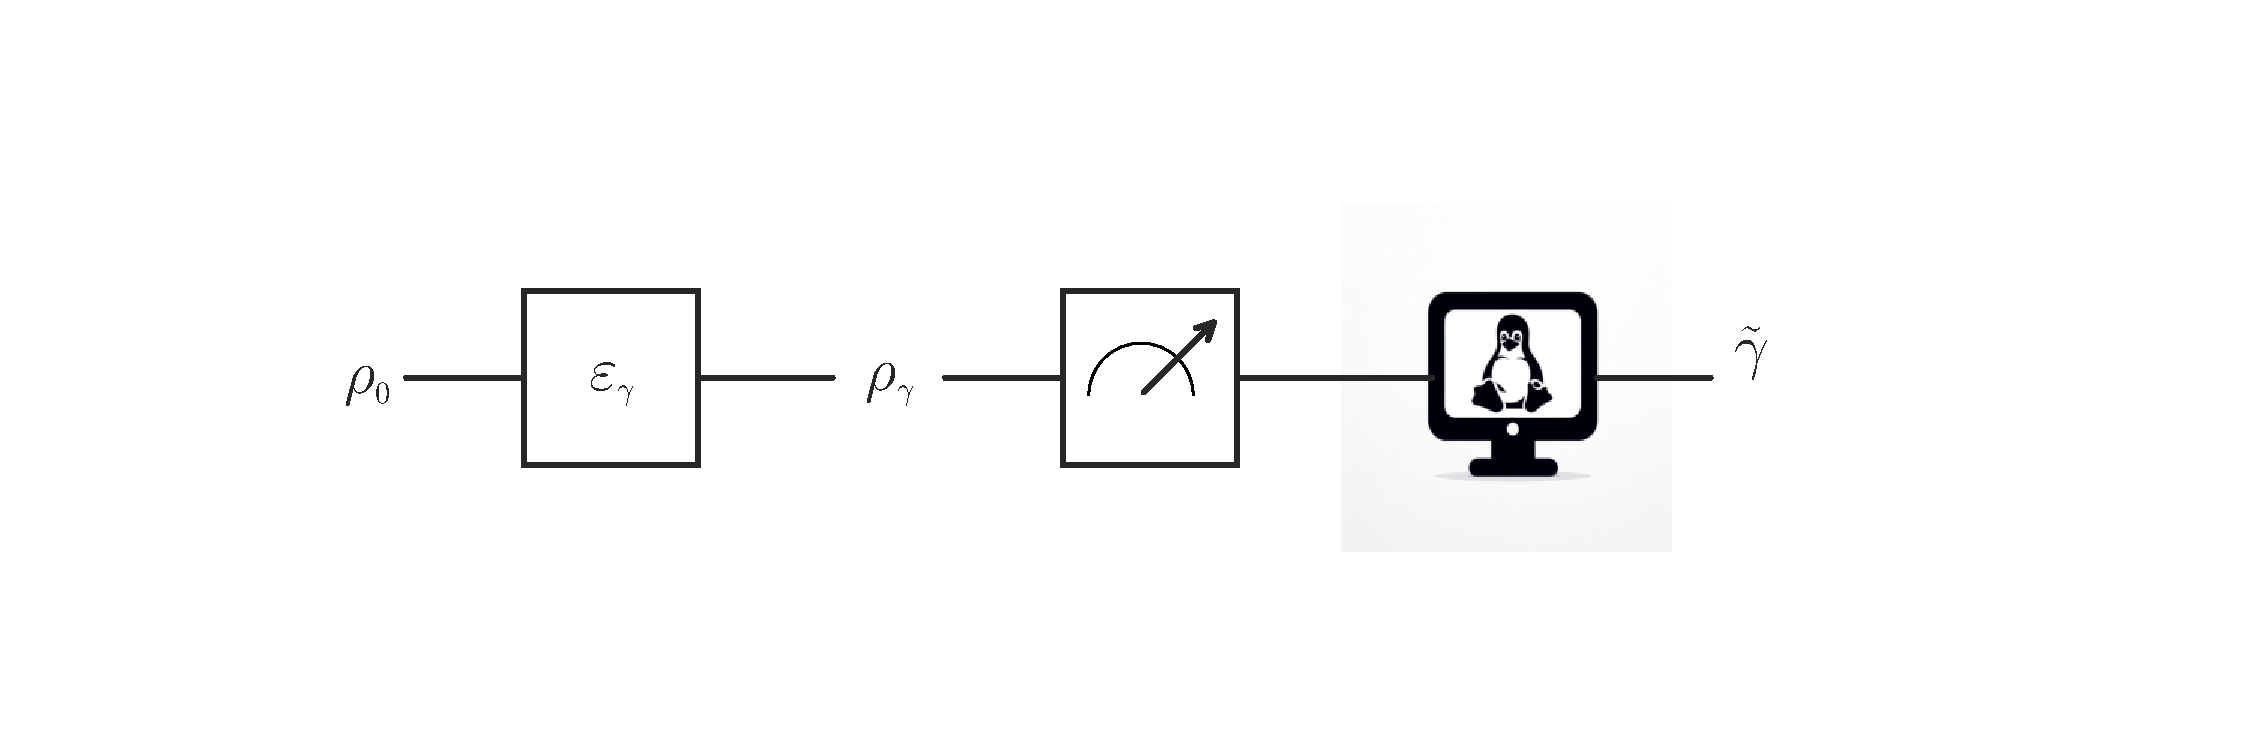
\includegraphics[scale=0.5]{CodeImages/Esquema_Estimacion.pdf}
  \caption{Schematic depiction of a metrology scheme}
  \label{fig:metrology_scheme}
\end{figure}

The objective of quantum metrology is to leverage the nonclassical
aspects of quantum theory to estimate as precisely as possible a
parameter of interest, given a fixed amount of certain
\textbf{resource} involved in the estimation.

\subsection{Optimal POVMs and Precision Bounds}
Different choices of measurement strategy will lead to different
distributions and in turn to different values of FI, this means
that not all the POVMs are made equal. A good
question now is wheter one can bound the FI for all possible
POVMs, this is indeed the case via a procedure proposed the
\cite{braunstein_statistical_1994} which we outline below.

\subsubsection{The Quantum Fisher Information}
Consider a generic metrology scheme as outlined at the beginning of
the section, the integrand in the FI heavily resembles a logarithmic derivative so taking
this as inspiration a new operator called the \textbf{Self-adjoint
  Logarithmic Derivative} (SLD) is introduced,  we define it as
a self-adjoint solution to the equation

\begin{equation}
  \partial_{\gamma}\rho_{\gamma} = \frac{1}{2}\left(\Lambda_{\gamma}\rho_{\gamma} + \rho_{\gamma}\Lambda_{\gamma} \right),
\end{equation}

later we'll come back to discuss its uniqueness and potential
problems that may arise. Using this we find:

\begin{align}
  \Tr{\Pi_{x}\partial_{\gamma}\rho_{\gamma}} =& \Re{\Tr{\Pi_{x}\rho_{\gamma}\Lambda_{\gamma}}}\\
   F(\gamma) =& \int dx\hspace{0.1cm} \frac{\Re{\Tr{\Pi_{x}\rho_{\gamma}\Lambda_{\gamma}}}^{2}}{\Tr{\Pi_{x}\rho_{\gamma}}}\\
   F(\gamma) \leq& \int dx\hspace{0.1cm} \frac{|\Tr{\Pi_{x}\rho_{\gamma}\Lambda_{\gamma}}|^{2}}{\Tr{\Pi_{x}\rho_{\gamma}}}\\
   F(\gamma) \leq& \int dx\hspace{0.1cm} \frac{\Tr{\sqrt{\Pi_{x}}\sqrt{\rho_{\gamma}}\sqrt{\rho_{\gamma}}\Lambda_{\gamma}\sqrt{\Pi_{x}}}}{\Tr{\Pi_{x}\rho_{\gamma}}}\\
\end{align}

Using the Cauchy-Schwartz inequality and the normalization of the POVM:

\begin{equation}
F(\gamma) \leq  \Tr{\rho_{\gamma}\Lambda_{\gamma}^{2}}.
\end{equation}
